\documentclass[sigconf]{acmart}
% use \code{foobar} for monospace (instead of \texttt{qux})
\newcommand{\code}{\texttt}

\usepackage{booktabs} % For formal tables
\usepackage{graphicx}
\usepackage[english]{babel}



\begin{document}
\settopmatter{printacmref=false} % Removes citation information below abstract
\renewcommand\footnotetextcopyrightpermission[1]{} % removes footnote with conference information in first column
\pagestyle{plain} % removes running headers

\title{Cryptocurrency Market Prediction Using Twitter}
\subtitle{Milestone 1 Update}

\author{Will Badart}
\affiliation{%
  \institution{University of Notre Dame}
  \city{South Bend}
  \state{Indiana}
}
\email{wbadart@nd.edu}

\author{Matthew Fabian}
\affiliation{%
  \institution{University of Notre Dame}
  \city{South Bend}
  \state{Indiana}
}
\email{mfabian1@nd.edu}

\author{Shane Ryan}
\affiliation{%
  \institution{University of Notre Dame}
  \city{South Bend}
  \state{Indiana}
}
\email{sryan8@nd.edu}

\author{Mara Staines}
\affiliation{%
  \institution{University of Notre Dame}
  \city{South Bend}
  \state{Indiana}
}
\email{mstaines@nd.edu}


\begin{abstract}
Cryptocurrency as a commodity has proven to be quite volatile, making prediction of market trends highly valuable. Our team will leverage the constant stream of tweets discussing cryptocurrency on Twitter in order to build a model that can predict changes in a cryptocurrency's value.
\end{abstract}

\maketitle


\section{Introduction}
Every day, Twitter users produce more than 500 million tweets\cite{sayce}. This makes Twitter an ideal resource for social sensing --- the use of humans as sensors. Users tweet and retweet about events, places, emotions, and more; the aggregation of this data has proven powerful for event detection and prediction. One of the fastest-growing conversations taking place on the platform is over cryptocurrency.

Cryptocurrency is a growing market that is both widely discussed and highly volatile, leading our team to believe that tweets may reflect trends in cryptocurrency value. Successfully using Twitter data to predict changes in cryptocurrency markets would provide a significant advantage in cryptocurrency trading. In this project, we will build a model to predict changes in the value of several major cryptocurrencies based on real-time data from Twitter.


\section{Approach}

\subsection{Data Sources}
Data for this project is collected from Twitter. We streamed tweets  using the Twitter API, which allows for tweets to be collected in near real-time. The filtering capability of the Twitter API allowed us to only collect tweets that contain certain keywords. We have selected both general keywords (e.g. \code{cryptocurrency}, \code{altcoin}) and keywords for the specific cryptocurrencies we will be exploring (e.g. \code{bitcoin}, \code{BTC}, \code{ethereum}). If a tweet contains one or more of these keywords, our program will store the tweet body as well as important metadata (user ID, timestamp, retweets, favorites, etc.) in JSON format and append it to a data file.

Many sites provide historical data on cryptocurrency value. We utilize the API of \href{https://www.cryptocompare.com}{CryptoCompare.com} to retrieve cryptocurrency values for the timespan of covered by the collected tweets.

\subsection{Methodology}

\begin{figure}[H]
\caption{Flow of data processing}
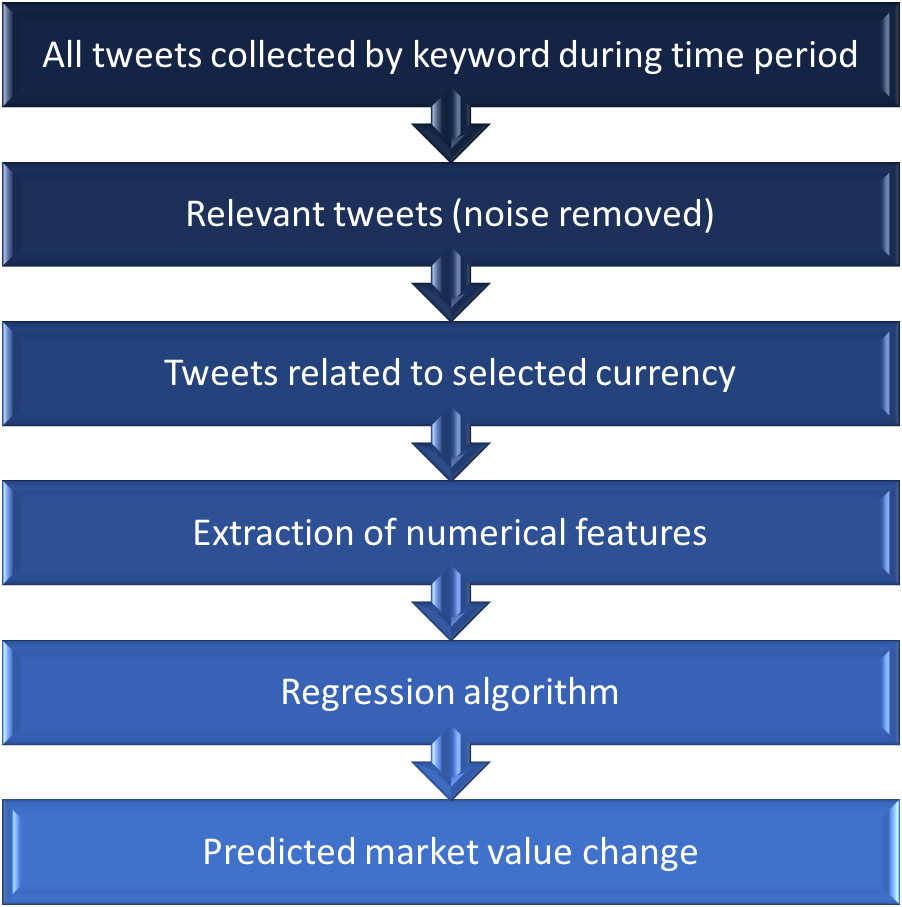
\includegraphics[width=7cm]{chart.png}
\end{figure}

Once data is collected from Twitter, it is be cleaned, categorized, and used in a regression model to make currency valule predictions (Figure 1). Twitter data is noisy, so the first component of data processing eliminates tweets irrelevant to cryptocurrency which made it past the API filter. Our strategy for this task is to use a clustering algorithm to group tweets as relevant or noise. The data is tokenized using the NLTK TweetTokenizer, which splits the tweet text into distinct words. This submodule is superior to simply splitting the data on whitespace, because it has been coded for the type of text encountered on Twitter. For example, it can split text to preserve common emoticons. The tokenized tweets are used to generate a matrix of token counts. The similarity of two tweets' token count vectors is the measurement used as distance in the clustering algorithm. Tweets are clustered using the KMeans algorithm. This algorithm fits the purpose well, as the number of clusters is known (n=2), and outliers are unlikely due to the character limit imposed on tweets. Our research has found that running KMeans on the data in multiple iterations progressively removes more irrelevant tweets, with the current optimal number of iterations at 3. Figure 2 shows a visual representation after the third iteration of clustering.

\begin{figure}[H]
\caption{Third Iteration of Relevant/Irrelevant Clustering}
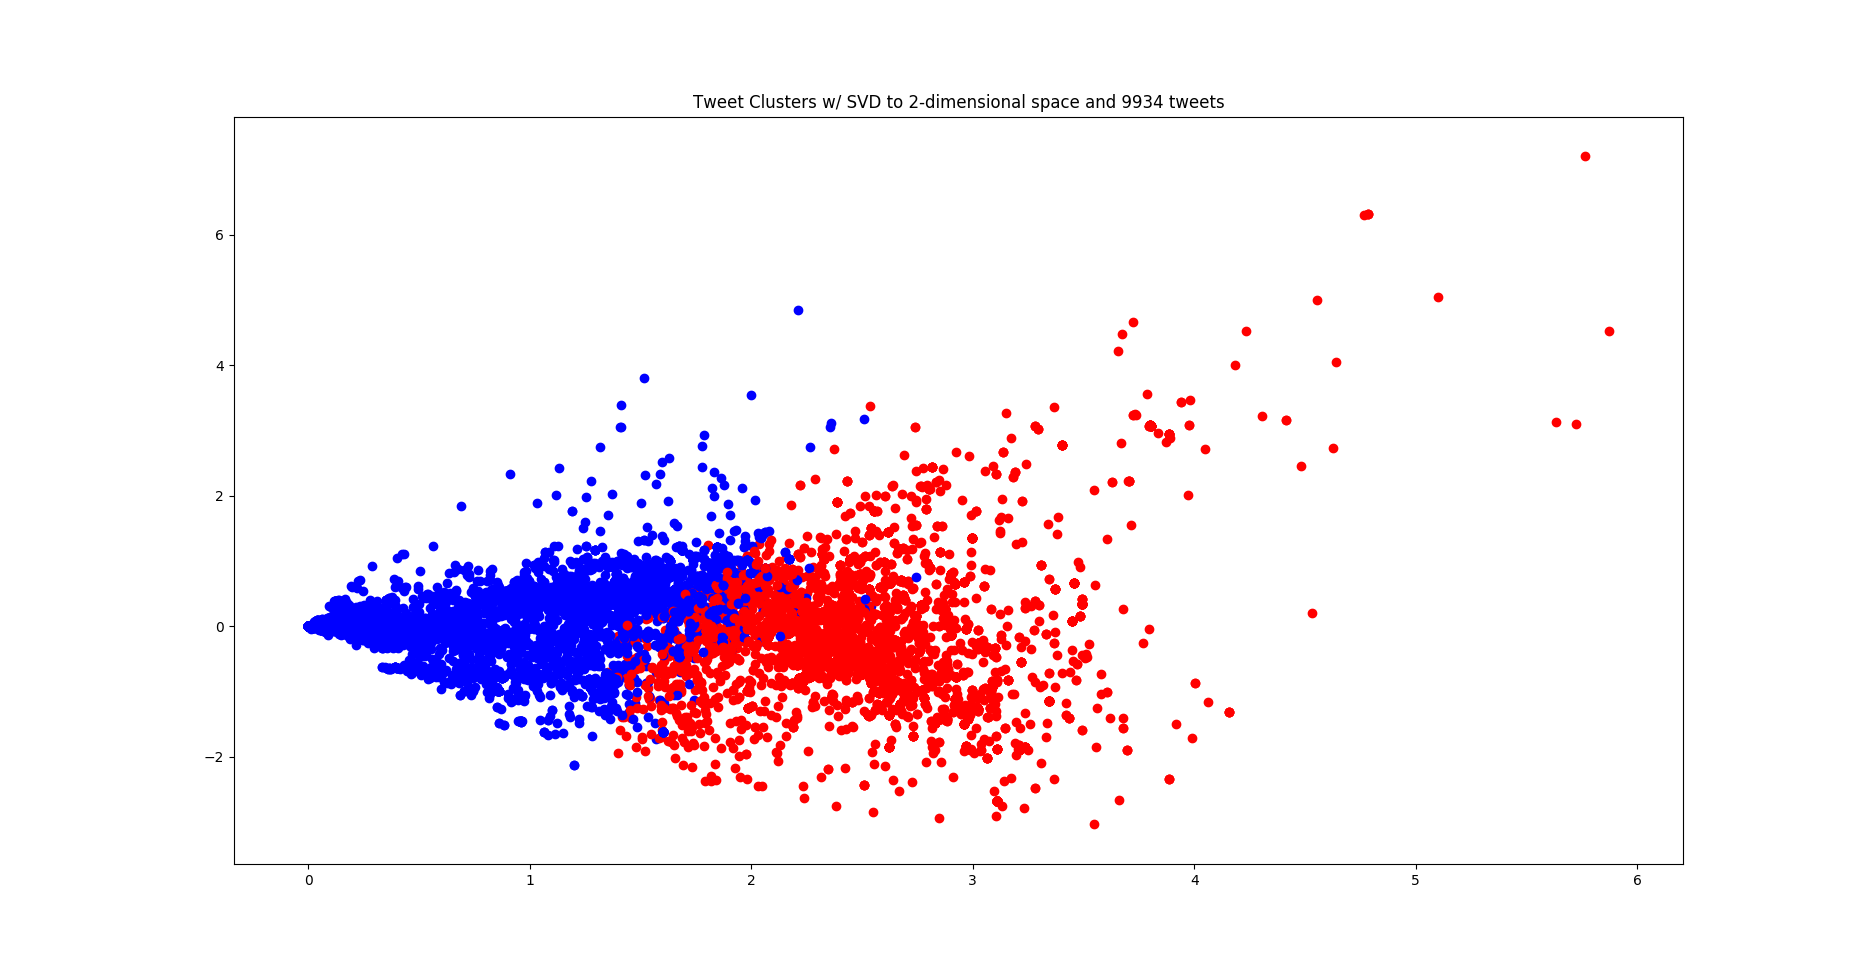
\includegraphics[width=9cm]{3pass.png}
\end{figure}

Once noise is removed and each tweet is labeled with the currency (or currencies) to which it refers, data from the tweets is used to calculate several features for use in the regression model. Features currently calculated for each timespan are number of tweets, average sentiment of tweets, and standard deviation of tweet sentiment. Sentiment is calculated using TextBlob, which relies on NLTK. The sentiment is a score from -1 to 1 (extremely negative to extremely positive). Standard deviation of sentiment aims to capture volatility in tweet content. Many neutral tweets would have an average sentiment of 0, as would equal numbers of highly positive and highly negative tweets. However, the standard deviation for netural tweets would be significantly smaller than that for tweets with opposing sentiment. 

Currently, due to constraints on time granularity when collecting historial currency prices, tweets are grouped by the hour to generate an instance and calculate its features. Before the final edits on this paper, we plan to have at least several days worth of data collected on the scale of minutes. This will allow us to test the limits of our model in predicting micro-trends.

The regression model is still in its early stages. We are currently using Ridge Regression for our model. Inital tests using 24 data points (1 day) could certainly be worse (Figure 3). The model shows little predictive ability (R-Squared = 0.04), but we are confident that with a larger data set (ideally 2 or more weeks) and improved features, the model will show significant improvement. We currently have over a month of data, but the processing pipeline to transform raw tweets into hourly datapoints is still being developed.

\begin{figure}[H]
\caption{Regression model given 24 data points for April 6}
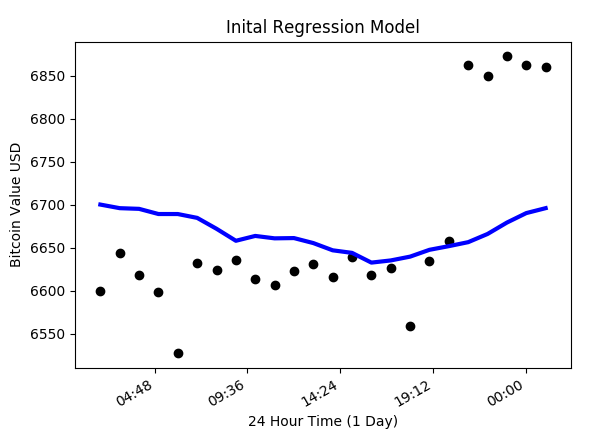
\includegraphics[width=7cm]{regression.png}
\end{figure}


\section{Results}
Evaluation for our model relies on knowing the ground truth: actual cryptocurrency values over time. Comparison of our predicted changes to actual changes is currently measured by $R^2$. We seek to maximize accuracy of our predictions and minimize the time needed to make a prediction. Currently, an hour worth of tweets provides very little predictive ability. However, for the scope of this course, a successful project will consist of a final model that can take an input period no longer than one day and output an accurate prediction of change in value for a currency.

The accuracy for our model's predictive ability can be measured in two ways: on historical data (for days for which we've collected tweets) and on current data. The first method involves building a model on historical data, then predicting the target value for the timespan immediately following te last data point. This prediction will be compared to the actual value from CryptoCompare.com. The second method, using current data, streams live data into the model, predicts the target value at the end of the data, then compares the predicted value to the true value once the time of the prediction is reached. The absolute difference between the model's output and CryptoCompare.com's report, $|value_c - value_m|$, can be interpreted as the model's performance.

\section{Discussion}

This research has presented several unique challenges. While Twitter data is plentiful, ensuring quality is difficult. First, technical resources must be chosen carefully to handle the extended, continuous uptime of a Twitter streaming program as well as the large files resulting from this stream. Because the data is temporal, missing a continuous chunk of data can hinder the model. In addition, it is difficult to extract quality text from Tweets. When we conceptualize Twitter, we think of our friends, family, and journalists sharing complete thoughts. In reality, a large number of tweets that are picked up by keyword filters are bots, scams, giveaways, or simply incoherent. With our desire to leverage tweet sentiment, removing this noise becomes extremely important. While we have made significant progress in removing irrelevant tweets, it is a difficult proccess. What makes a tweet irrelevant is not clear cut, and we do not have any access to ground truths. For the final edits to this paper, the results section will include by-hand validation of 100-500 of the tweets clustered by KMeans, in order to provide a more quantitative sense of model performance. This project has been a great experience because in the real world, data is messy, noisy, and incomplete. Developing strategies to still find value in this data has helped us all grow immensely over the course of the semester.

\bibliographystyle{ACM-Reference-Format}
\bibliography{milestone}

\end{document}
